% Graph generated from dotgraph.rb with heavy help from dot2tex.
% DotGraph#to_tex(:figonly=>true, :attrs=>["overlap=false", "splines=true", "node [fixedsize, style=\"ball color=blue!15, semitransparent\"]", "edge [len=2]"], :texmode=>"raw", :fmt=>"tikz", :alg=>:neato, :graphstyle=>"scale=0.7", :exp=>0.2)
% This called:
% dot2tex --prog=neato --figonly --graphstyle="scale=0.7" -traw
% 
%
% You may need the following packages:
% \usepackage[x11names, rgb]{xcolor}
% \usepackage{tikz}
% \usetikzlibrary{snakes,arrows,shapes}


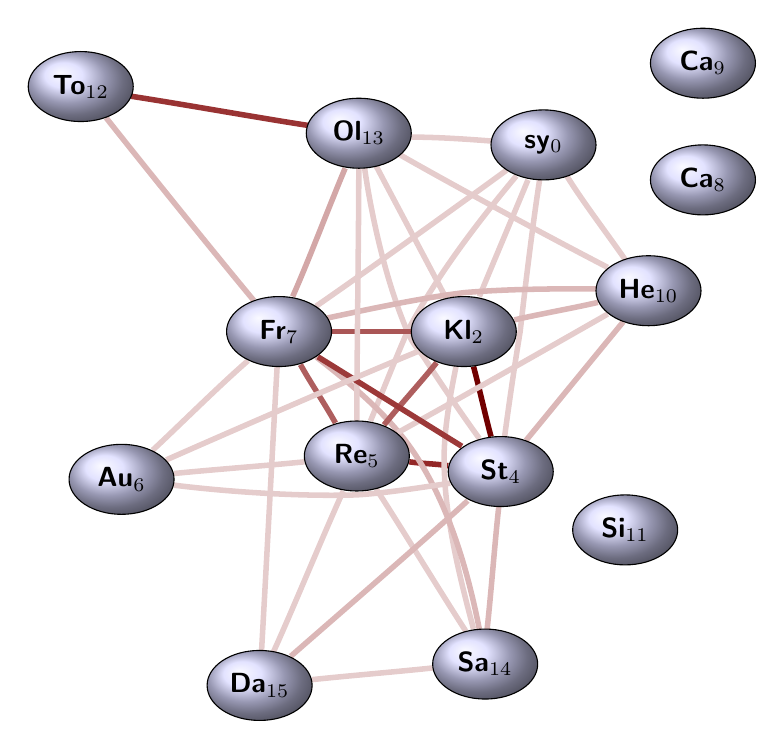
\begin{tikzpicture}[>=latex,join=bevel,scale=0.7]
%  \pgfsetlinewidth{1bp}
%%
\pgfsetcolor{black}
  % Edge: u5 -- u0
  \draw [color=black!50!red!20.0,line width=2] (177bp,155bp) .. controls (182bp,167bp) and (189bp,185bp)  .. (196bp,201bp) .. controls (212bp,232bp) and (237bp,263bp)  .. (252bp,281bp);
  % Edge: u15 -- u7
  \draw [color=black!50!red!20.0,line width=2] (121bp,37bp) .. controls (123bp,72bp) and (127bp,148bp)  .. (129bp,183bp);
  % Edge: u13 -- u4
  \draw [color=black!50!red!20.0,line width=2] (174bp,285bp) .. controls (177bp,264bp) and (184bp,229bp)  .. (196bp,201bp) .. controls (199bp,194bp) and (201bp,193bp)  .. (205bp,187bp) .. controls (214bp,173bp) and (225bp,157bp)  .. (233bp,146bp);
  % Edge: u7 -- u2
  \draw [color=black!50!red!66.332495807108,line width=2] (157bp,201bp) .. controls (170bp,201bp) and (185bp,201bp)  .. (198bp,201bp);
  % Edge: u5 -- u4
  \draw [color=black!50!red!84.8528137423857,line width=2] (197bp,134bp) .. controls (204bp,133bp) and (211bp,133bp)  .. (217bp,132bp);
  % Edge: u7 -- u6
  \draw [color=black!50!red!20.0,line width=2] (114bp,186bp) .. controls (99bp,173bp) and (79bp,153bp)  .. (65bp,140bp);
  % Edge: u13 -- u0
  \draw [color=black!50!red!20.0,line width=2] (198bp,301bp) .. controls (211bp,301bp) and (226bp,300bp)  .. (239bp,299bp);
  % Edge: u14 -- u2
  \draw [color=black!50!red!20.0,line width=2] (230bp,48bp) .. controls (225bp,67bp) and (216bp,100bp)  .. (215bp,129bp) .. controls (214bp,147bp) and (218bp,168bp)  .. (221bp,183bp);
  % Edge: u4 -- u10
  \draw [color=black!50!red!28.2842712474619,line width=2] (257bp,145bp) .. controls (271bp,162bp) and (293bp,189bp)  .. (307bp,206bp);
  % Edge: u7 -- u5
  \draw [color=black!50!red!63.2455532033676,line width=2] (141bp,184bp) .. controls (146bp,175bp) and (154bp,163bp)  .. (159bp,154bp);
  % Edge: u13 -- u12
  \draw [color=black!50!red!80.0,line width=2] (145bp,307bp) .. controls (119bp,311bp) and (80bp,318bp)  .. (54bp,322bp);
  % Edge: u4 -- u2
  \draw [color=black!50!red!111.3552872566,line width=2] (239bp,147bp) .. controls (236bp,158bp) and (233bp,172bp)  .. (230bp,183bp);
  % Edge: u14 -- u7
  \draw [color=black!50!red!28.2842712474619,line width=2] (233bp,48bp) .. controls (228bp,73bp) and (217bp,120bp)  .. (190bp,151bp) .. controls (178bp,165bp) and (162bp,178bp)  .. (149bp,188bp);
  % Edge: u10 -- u0
  \draw [color=black!50!red!20.0,line width=2] (308bp,238bp) .. controls (299bp,251bp) and (286bp,268bp)  .. (278bp,281bp);
  % Edge: u13 -- u7
  \draw [color=black!50!red!34.6410161513775,line width=2] (164bp,285bp) .. controls (156bp,266bp) and (145bp,237bp)  .. (137bp,219bp);
  % Edge: u5 -- u2
  \draw [color=black!50!red!63.2455532033676,line width=2] (184bp,153bp) .. controls (192bp,163bp) and (203bp,175bp)  .. (211bp,185bp);
  % Edge: u5 -- u10
  \draw [color=black!50!red!20.0,line width=2] (191bp,149bp) .. controls (220bp,165bp) and (271bp,194bp)  .. (299bp,210bp);
  % Edge: u2 -- u0
  \draw [color=black!50!red!20.0,line width=2] (233bp,219bp) .. controls (240bp,236bp) and (251bp,262bp)  .. (258bp,279bp);
  % Edge: u15 -- u14
  \draw [color=black!50!red!20.0,line width=2] (147bp,22bp) .. controls (166bp,24bp) and (190bp,26bp)  .. (209bp,28bp);
  % Edge: u14 -- u4
  \draw [color=black!50!red!28.2842712474619,line width=2] (237bp,48bp) .. controls (239bp,66bp) and (241bp,93bp)  .. (243bp,111bp);
  % Edge: u7 -- u0
  \draw [color=black!50!red!20.0,line width=2] (149bp,214bp) .. controls (175bp,232bp) and (221bp,265bp)  .. (247bp,284bp);
  % Edge: u6 -- u4
  \draw [color=black!50!red!20.0,line width=2] (76bp,122bp) .. controls (100bp,119bp) and (138bp,116bp)  .. (170bp,117bp) .. controls (186bp,118bp) and (204bp,121bp)  .. (218bp,123bp);
  % Edge: u15 -- u5
  \draw [color=black!50!red!20.0,line width=2] (127bp,36bp) .. controls (137bp,58bp) and (153bp,97bp)  .. (163bp,119bp);
  % Edge: u13 -- u10
  \draw [color=black!50!red!20.0,line width=2] (192bp,292bp) .. controls (220bp,276bp) and (270bp,249bp)  .. (299bp,234bp);
  % Edge: u13 -- u2
  \draw [color=black!50!red!20.0,line width=2] (180bp,286bp) .. controls (190bp,267bp) and (206bp,237bp)  .. (216bp,218bp);
  % Edge: u4 -- u0
  \draw [color=black!50!red!20.0,line width=2] (246bp,147bp) .. controls (248bp,162bp) and (251bp,183bp)  .. (254bp,201bp) .. controls (257bp,228bp) and (261bp,260bp)  .. (264bp,279bp);
  % Edge: u14 -- u5
  \draw [color=black!50!red!20.0,line width=2] (226bp,47bp) .. controls (213bp,67bp) and (193bp,100bp)  .. (180bp,120bp);
  % Edge: u6 -- u5
  \draw [color=black!50!red!20.0,line width=2] (76bp,128bp) .. controls (96bp,130bp) and (123bp,132bp)  .. (143bp,134bp);
  % Edge: u15 -- u4
  \draw [color=black!50!red!28.2842712474619,line width=2] (136bp,34bp) .. controls (160bp,55bp) and (204bp,93bp)  .. (227bp,114bp);
  % Edge: u7 -- u10
  \draw [color=black!50!red!28.2842712474619,line width=2] (155bp,208bp) .. controls (174bp,212bp) and (201bp,218bp)  .. (225bp,221bp) .. controls (248bp,223bp) and (274bp,223bp)  .. (293bp,223bp);
  % Edge: u13 -- u5
  \draw [color=black!50!red!20.0,line width=2] (171bp,285bp) .. controls (171bp,253bp) and (170bp,187bp)  .. (170bp,155bp);
  % Edge: u12 -- u7
  \draw [color=black!50!red!28.2842712474619,line width=2] (41bp,311bp) .. controls (60bp,287bp) and (97bp,241bp)  .. (117bp,217bp);
  % Edge: u7 -- u4
  \draw [color=black!50!red!77.4596669241483,line width=2] (150bp,188bp) .. controls (171bp,175bp) and (203bp,155bp)  .. (224bp,142bp);
  % Edge: u10 -- u2
  \draw [color=black!50!red!28.2842712474619,line width=2] (294bp,216bp) .. controls (281bp,213bp) and (264bp,210bp)  .. (251bp,207bp);
  % Edge: u6 -- u2
  \draw [color=black!50!red!20.0,line width=2] (72bp,135bp) .. controls (106bp,150bp) and (168bp,177bp)  .. (202bp,191bp);
  % Node: u9
\begin{scope}
  \pgfsetstrokecolor{black}
  \draw [ball color=blue!15] (348bp,339bp) ellipse (27bp and 18bp);
  \draw (348bp,339bp) node {\textbf{\textsf{Ca}}$_{9}$};
\end{scope}
  % Node: u8
\begin{scope}
  \pgfsetstrokecolor{black}
  \draw [ball color=blue!15] (348bp,279bp) ellipse (27bp and 18bp);
  \draw (348bp,279bp) node {\textbf{\textsf{Ca}}$_{8}$};
\end{scope}
  % Node: u5
\begin{scope}
  \pgfsetstrokecolor{black}
  \draw [ball color=blue!15] (170bp,137bp) ellipse (27bp and 18bp);
  \draw (170bp,137bp) node {\textbf{\textsf{Re}}$_{5}$};
\end{scope}
  % Node: u4
\begin{scope}
  \pgfsetstrokecolor{black}
  \draw [ball color=blue!15] (244bp,129bp) ellipse (27bp and 18bp);
  \draw (244bp,129bp) node {\textbf{\textsf{St}}$_{4}$};
\end{scope}
  % Node: u7
\begin{scope}
  \pgfsetstrokecolor{black}
  \draw [ball color=blue!15] (130bp,201bp) ellipse (27bp and 18bp);
  \draw (130bp,201bp) node {\textbf{\textsf{Fr}}$_{7}$};
\end{scope}
  % Node: u6
\begin{scope}
  \pgfsetstrokecolor{black}
  \draw [ball color=blue!15] (49bp,125bp) ellipse (27bp and 18bp);
  \draw (49bp,125bp) node {\textbf{\textsf{Au}}$_{6}$};
\end{scope}
  % Node: u0
\begin{scope}
  \pgfsetstrokecolor{black}
  \draw [ball color=blue!15] (266bp,297bp) ellipse (27bp and 18bp);
  \draw (266bp,297bp) node {\textbf{\textsf{sy}}$_{0}$};
\end{scope}
  % Node: u2
\begin{scope}
  \pgfsetstrokecolor{black}
  \draw [ball color=blue!15] (225bp,201bp) ellipse (27bp and 18bp);
  \draw (225bp,201bp) node {\textbf{\textsf{Kl}}$_{2}$};
\end{scope}
  % Node: u11
\begin{scope}
  \pgfsetstrokecolor{black}
  \draw [ball color=blue!15] (308bp,99bp) ellipse (27bp and 18bp);
  \draw (308bp,99bp) node {\textbf{\textsf{Si}}$_{11}$};
\end{scope}
  % Node: u10
\begin{scope}
  \pgfsetstrokecolor{black}
  \draw [ball color=blue!15] (320bp,222bp) ellipse (27bp and 18bp);
  \draw (320bp,222bp) node {\textbf{\textsf{He}}$_{10}$};
\end{scope}
  % Node: u13
\begin{scope}
  \pgfsetstrokecolor{black}
  \draw [ball color=blue!15] (171bp,303bp) ellipse (27bp and 18bp);
  \draw (171bp,303bp) node {\textbf{\textsf{Ol}}$_{13}$};
\end{scope}
  % Node: u12
\begin{scope}
  \pgfsetstrokecolor{black}
  \draw [ball color=blue!15] (28bp,327bp) ellipse (27bp and 18bp);
  \draw (28bp,327bp) node {\textbf{\textsf{To}}$_{12}$};
\end{scope}
  % Node: u15
\begin{scope}
  \pgfsetstrokecolor{black}
  \draw [ball color=blue!15] (120bp,19bp) ellipse (27bp and 18bp);
  \draw (120bp,19bp) node {\textbf{\textsf{Da}}$_{15}$};
\end{scope}
  % Node: u14
\begin{scope}
  \pgfsetstrokecolor{black}
  \draw [ball color=blue!15] (236bp,30bp) ellipse (27bp and 18bp);
  \draw (236bp,30bp) node {\textbf{\textsf{Sa}}$_{14}$};
\end{scope}
%
\end{tikzpicture}


%%% Local Variables: 
%%% mode: latex
%%% TeX-master: "tutorial"
%%% End: 
